% Created 2016-04-10 日 22:01
\documentclass[xcolor=svgnames,presentation]{beamer}
\usepackage[utf8]{inputenc}
\usepackage[T1]{fontenc}
\usepackage{fixltx2e}
\usepackage{graphicx}
\usepackage{longtable}
\usepackage{float}
\usepackage{wrapfig}
\usepackage{soul}
\usepackage{textcomp}
\usepackage{marvosym}
\usepackage{wasysym}
\usepackage{latexsym}
\usepackage{amssymb}
\usepackage{hyperref}
\tolerance=1000
\usepackage{minted}
\usecolortheme[named=FireBrick]{structure}\setbeamercovered{transparent}\setbeamertemplate{caption}[numbered]\setbeamertemplate{blocks}[rounded][shadow=true] \usetheme{Darmstadt}\date{\today} \usepackage{tikz}\usepackage{xeCJK}\usepackage{amsmath}\setmainfont{Times New Roman}\setCJKmainfont[BoldFont={Adobe Heiti Std},ItalicFont={Adobe Fangsong Std}]{Adobe Heiti Std}\setCJKsansfont{Adobe Heiti Std}\setCJKmonofont{Adobe Fangsong Std}\usepackage{verbatim}\graphicspath{{figures/}} \definecolor{lstbgcolor}{rgb}{0.9,0.9,0.9} \usepackage{listings}\usepackage{minted} \usepackage{fancyvrb}\usepackage{xcolor}\lstset{escapeinside=`',frameround=ftft,language=C,breaklines=true,keywordstyle=\color{blue!70},commentstyle=\color{red!50!green!50!blue!50},frame=shadowbox,backgroundcolor=\color{yellow!20},rulesepcolor=\color{red!20!green!20!blue!20}}
\usemintedstyle{default}
\providecommand{\alert}[1]{\textbf{#1}}

\title{第5讲 Shell脚本编程}
\author{王晓庆}
\date{\today}
\hypersetup{
  pdfkeywords={},
  pdfsubject={},
  pdfcreator={Emacs Org-mode version 7.9.3f}}

\institute{wangxiaoqing@outlook.com}
\begin{document}

\maketitle

\begin{frame}
\frametitle{Outline}
\setcounter{tocdepth}{1}
\tableofcontents
\end{frame}

\section{shell脚本编程}
\label{sec-1}
\subsection{入门}
\label{sec-1-1}
\begin{frame}[fragile]
\frametitle{创建新命令}
\label{sec-1-1-1}
\begin{exampleblock}{示例:统计当前有多少不同用户在线}
\label{sec-1-1-1-1}


\begin{minted}[]{bash}
who | cut -d" " -f1 | sort | uniq | wc -l
#如需反复执行上述命令,则可以将其组织成一个新命令
echo 'who | cut -d" " -f1 | sort | uniq | wc -l' >nu
#执行
1. sh <nu
2. sh nu
3. chmod +x nu
   ./nu
4. mkdir bin
   echo $PATH
   mv nu bin
   ls nu
   nu
\end{minted}
\end{exampleblock}
\end{frame}
\begin{frame}[fragile]
\frametitle{命令参数}
\label{sec-1-1-2}
\begin{exampleblock}{示例:创建名为cx的程序,为文件设置可执行权}
\label{sec-1-1-2-1}


\begin{minted}[]{bash}
cx nu    #相当于chmod +x nu的缩写
#问题:如何为cx传递文件名参数?
echo 'chmod +x $1' >cx
sh cx cx
mv cx bin
echo echo Hi, there >hello
cx hello
./hello
#问题:如何处理多个参数?
chmod +x $1 $2 $3 $4 $5 $6 $7 $8 $9
chmod +x $*
echo 'wc -l $*' >lc
cx lc; mv lc bin
lc vim*
\end{minted}
\end{exampleblock}
\end{frame}
\begin{frame}[fragile]
\frametitle{命令参数}
\label{sec-1-1-3}
\begin{itemize}

\item shell脚本的参数不一定是文件名
\label{sec-1-1-3-1}%
\end{itemize} % ends low level
\begin{exampleblock}{示例:}
\label{sec-1-1-3-2}


\begin{verbatim}
假设文件/usr/share/phone-book保存了个人电话目录:
dial-a-joke 212-976-3838
dial-a-prayer 212-246-4200
dial santa 212-976-3636
dow jones report 212-976-4141
现在需要创建一个查号程序411:
echo 'grep $* /usr/share/phone-book' >411
cx 411; mv 411 bin
411 joke            #:-)
4111 'dow jones'    #:-(
\end{verbatim}
\end{exampleblock}
\note{解决办法

echo `grep -i ``\$*'' /usr/share/phone-book' >411
411 dow jones    \#:-)
}
\end{frame}
\begin{frame}[fragile]
\frametitle{I节点}
\label{sec-1-1-4}
\begin{itemize}

\item 一个文件包含:文件名、内容及管理信息(如权限、修改时间、文件长度、文件内容的存放位置等)
\label{sec-1-1-4-1}%

\item 文件的管理信息存放在I节点中,可以认为I节点就是文件,文件的系统内部名称就是它的I节点号。
\label{sec-1-1-4-2}%
\end{itemize} % ends low level
\begin{exampleblock}{示例}
\label{sec-1-1-4-3}


\begin{minted}[]{bash}
date >junk
ls -i junk       #查看文件的I节点号
ls -l junk       #显示最近修改(写)时间
cat junk
ls -lu junk      #显示最近访问(读/执行)时间
ls -lc junk      #显示最近修改I节点(如设置权限)时间
chmod 444 junk
ls -lc junk
\end{minted}
\end{exampleblock}
\end{frame}
\begin{frame}
\frametitle{I节点}
\label{sec-1-1-5}
\begin{itemize}

\item 目录、文件及I节点的关系如下图所示:\\
\label{sec-1-1-5-1}%
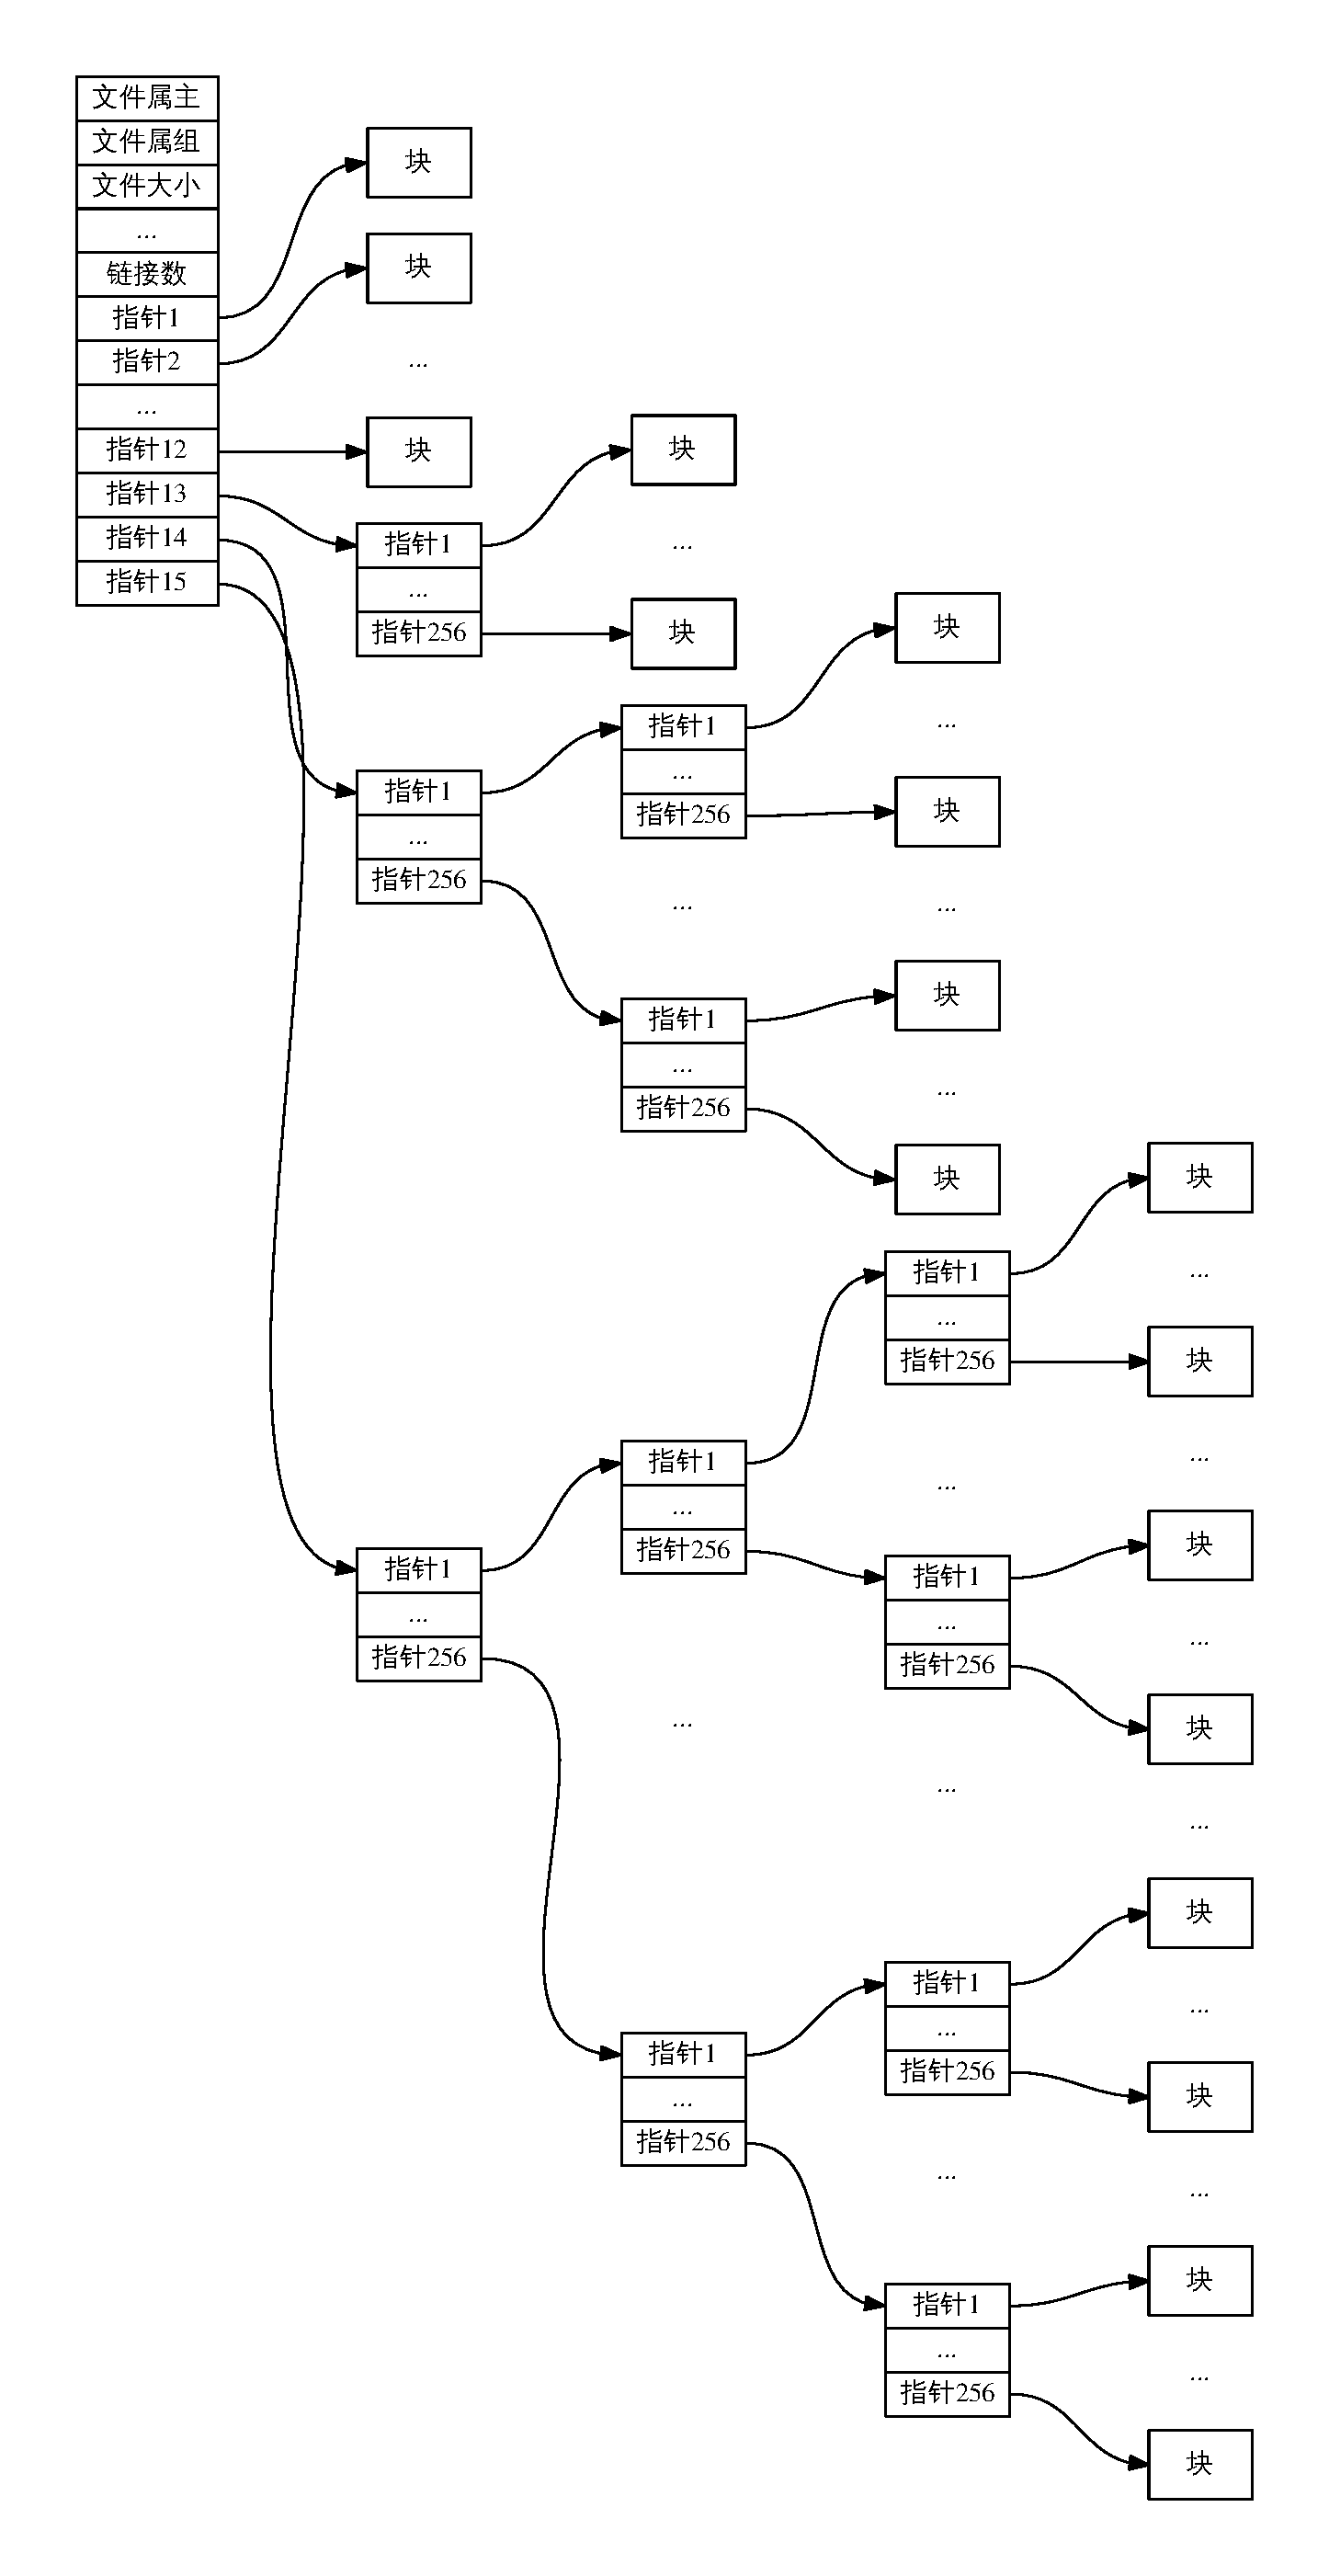
\includegraphics[width=.9\linewidth]{img/inode2.pdf}

\item 目录中的文件名被称作链,因为它把目录层次结构中的名称链接到它的I节点,因而也就链接到数据。
\label{sec-1-1-5-2}%

\item 同一个I节点号可以出现在多个目录项中
\label{sec-1-1-5-3}%

\item rm命令并不真正删除I节点,它删除目录入口或链,只有当链接到文件的最后链消失后,系统才删除文件本身。
\label{sec-1-1-5-4}%
\end{itemize} % ends low level
\end{frame}
\begin{frame}[fragile]
\frametitle{链接}
\label{sec-1-1-6}
\begin{itemize}

\item 创建硬链接\\
\label{sec-1-1-6-1}%
\begin{minted}[]{bash}
ln junk junk2
\end{minted}
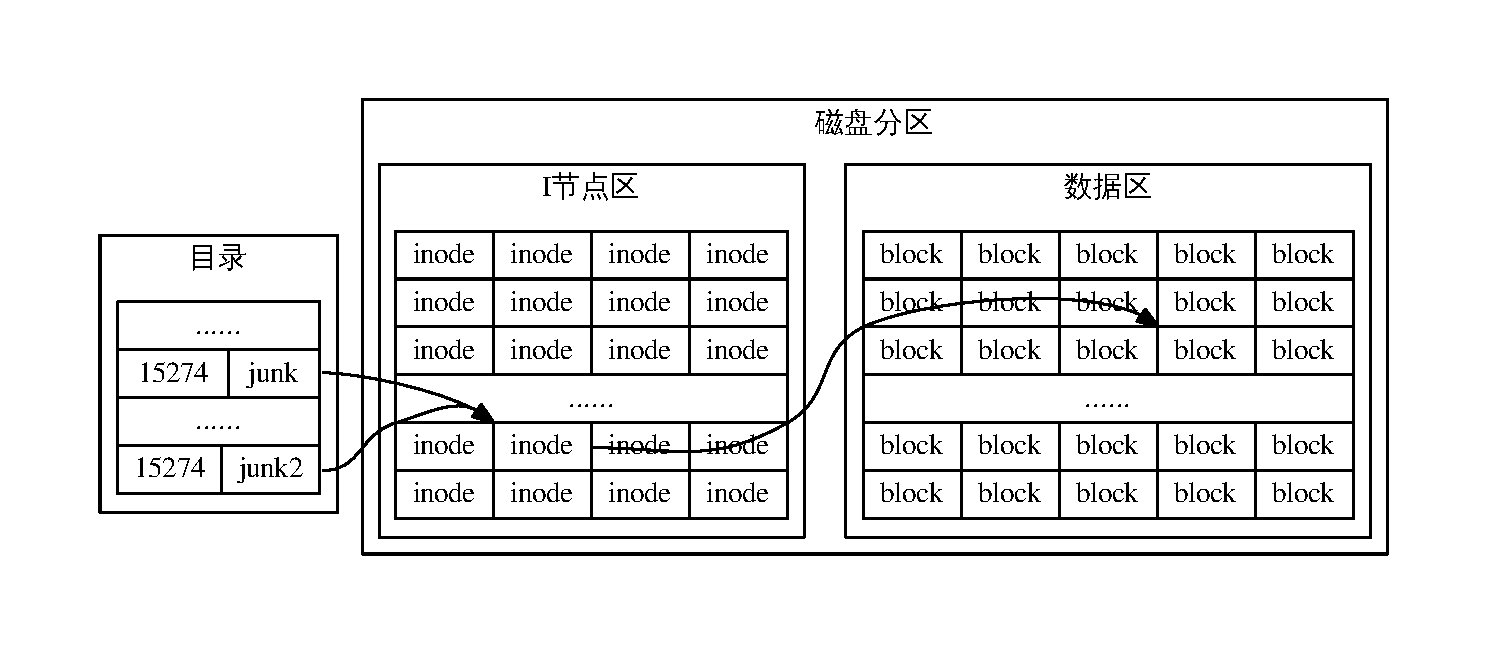
\includegraphics[width=.9\linewidth]{img/inode3.pdf}
\begin{itemize}

\item 不能跨文件系统创建硬链接
\label{sec-1-1-6-1-1}%

\item 不能为目录创建硬链接
\label{sec-1-1-6-1-2}%
\end{itemize} % ends low level
\end{itemize} % ends low level
\end{frame}
\begin{frame}[fragile]
\frametitle{链接}
\label{sec-1-1-7}
\begin{itemize}

\item 创建符号(软)链接\\
\label{sec-1-1-7-1}%
\begin{minted}[]{bash}
ln -s junk2 junk3
\end{minted}
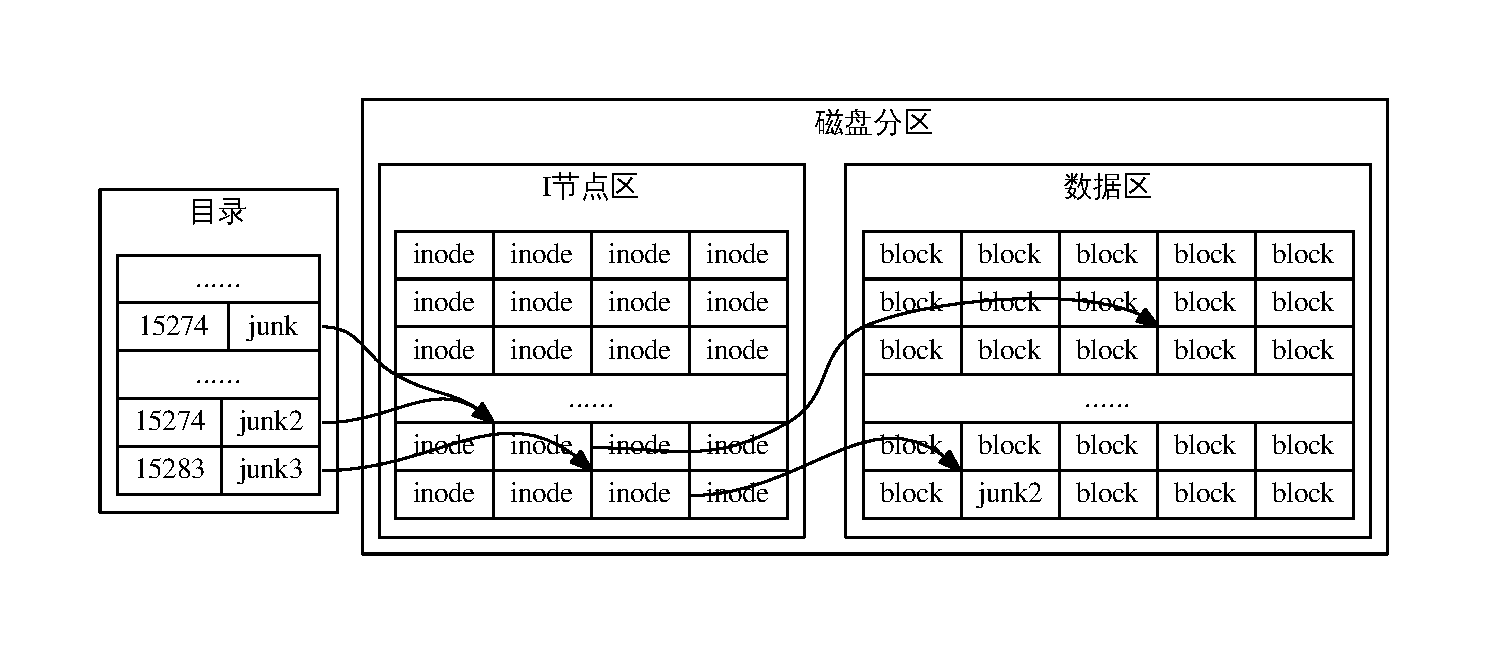
\includegraphics[width=.9\linewidth]{img/inode4.pdf}
\begin{itemize}

\item 符号链接保存的是路径(相对路径/绝对路径)
\label{sec-1-1-7-1-1}%

\item 符号链接依赖于其目标文件
\label{sec-1-1-7-1-2}%
\end{itemize} % ends low level
\end{itemize} % ends low level
\end{frame}
\begin{frame}
\frametitle{链接}
\label{sec-1-1-8}
\begin{block}{试一试}
\label{sec-1-1-8-1}

假设mike的主目录下有一个文件scratch,能否在mary的主目录下为该文件建立一个硬链接,使得mike和mary能够共享该文件?
\end{block}
\end{frame}
\begin{frame}[fragile]
\frametitle{命令参数}
\label{sec-1-1-9}
\begin{itemize}

\item 参数\$0是指正在执行的程序的名字
\label{sec-1-1-9-1}%
\end{itemize} % ends low level
\begin{exampleblock}{示例:将输入进行多列打印}
\label{sec-1-1-9-2}


\begin{minted}[]{bash}
ls | pr -t -5 #将输入按5列输出
echo 'pr -t -5' >5
cx 5; mv 5 bin
ls | 5
若要按2列、3列、4列、6列输出呢?
echo 'pr -t -$0' >5
ln 5 2;ln 5 3;ln 5 4;ln 5 6
ls | 5        #:-(
\end{minted}
\end{exampleblock}
\end{frame}
\begin{frame}[fragile]
\frametitle{程序输出作为参数}
\label{sec-1-1-10}
\begin{exampleblock}{前面的程序有什么问题呢?}
\label{sec-1-1-10-1}


\begin{minted}[]{bash}
vim 5
echo pr -t -$0 #调试技巧:将命令语句打印出来
ls | 5
vim 5
pr -t -`basename $0`  #反引号:命令替换
ls | 5
\end{minted}
\end{exampleblock}
\begin{block}{命令替换}
\label{sec-1-1-10-2}


\begin{minted}[]{bash}
#打印命令cat所在的目录
echo `dirname \`which cat\``
echo $(dirname $(which cat))
\end{minted}
\end{block}
\end{frame}
\begin{frame}[fragile]
\frametitle{shell变量}
\label{sec-1-1-11}
\begin{itemize}

\item set命令可以查看所有变量的值
\label{sec-1-1-11-1}%

\item 一个变量的值与创建它的shell有关,其值并不会自动传递给子shell
\label{sec-1-1-11-2}%
\end{itemize} % ends low level
\begin{exampleblock}{示例}
\label{sec-1-1-11-3}


\begin{minted}[]{bash}
x=Hello   #变量无需声明,注意:=两边不能有空格!
sh        #进入子shell
echo $x
Ctrl-d    #离开子shell
echo $x
#因为shell脚本是由子shell运行的,所以不能修改变量的值
echo -e 'x="Bye"\necho $x' >setx
sh setx
echo $x
\end{minted}
\end{exampleblock}
\end{frame}
\begin{frame}[fragile]
\frametitle{行内赋值}
\label{sec-1-1-12}
\begin{itemize}

\item 行内赋值可用于临时改变变量的值并传给脚本
\label{sec-1-1-12-1}%
\end{itemize} % ends low level
\begin{exampleblock}{示例}
\label{sec-1-1-12-2}


\begin{minted}[]{bash}
echo 'echo $x' >echox
cx echox;mv echox bin
x=300
x=500 echox
echo $x
\end{minted}
\end{exampleblock}
\end{frame}
\begin{frame}[fragile]
\frametitle{在当前shell中执行shell脚本}
\label{sec-1-1-13}
\begin{itemize}

\item 能否想办法用shell脚本来改变shell变量的值?
\label{sec-1-1-13-1}%
\end{itemize} % ends low level
\begin{exampleblock}{示例}
\label{sec-1-1-13-2}


\begin{minted}[]{bash}
echo $PATH
echo 'PATH=$PATH:/sbin' >>.bash_profile
sh .bash_profile
echo $PATH
. .bash_profile
echo $PATH
\end{minted}
\end{exampleblock}
\begin{block}{说明}
\label{sec-1-1-13-3}


\begin{minted}[]{bash}
source命令与.命令的意义相同:
source .bash_profile
\end{minted}
\end{block}
\end{frame}
\begin{frame}[fragile]
\frametitle{here文档(1)}
\label{sec-1-1-14}
\begin{itemize}

\item here文档:把命令的标准输入和命令放在一起
\label{sec-1-1-14-1}%
\end{itemize} % ends low level
\begin{exampleblock}{示例1}
\label{sec-1-1-14-2}


\begin{minted}[]{bash}
cat 411
grep "$*" <<End
dial-a-joke 212-976-3838
dial-a-prayer 212-246-4200
dial santa 212-976-3636
dow jones report 212-976-4141
End
#End(可自行选取其他单词)用于开始和终止输入(here文档)
#          <<End: here文档内的$、``和\会被替换
#<<\End和<<'End': here文档内的$、``和\不被替换
\end{minted}
\end{exampleblock}
\end{frame}
\begin{frame}[fragile]
\frametitle{here文档(2)}
\label{sec-1-1-15}
\begin{exampleblock}{示例2}
\label{sec-1-1-15-1}


\begin{minted}[]{bash}
cat avi
#!/bin/bash
if [ "$#" -ne 1 ]; then
  echo "Usage: avi file" 1>&2; exit 1
fi
vi $1 &>/dev/null <<EOF
iTo be or not to be,
It is a problem.^[
ZZ
EOF
#注意:^[代表ESC键,需先按C-v,再按ESC进行输入
avi problem  #执行avi
\end{minted}
\end{exampleblock}
\end{frame}
\begin{frame}[fragile]
\frametitle{循环}
\label{sec-1-1-16}
\begin{exampleblock}{基本的for循环}
\label{sec-1-1-16-1}


\begin{minted}[]{bash}
#多行
for i in a "b c" d
do
  echo $i
done
#单行
for i in a 'b c' d; do echo $i; done
#通过命令生成列表
for i in `seq 10 20`; do
  echo $i
done
\end{minted}
\end{exampleblock}
\end{frame}
\begin{frame}[fragile]
\frametitle{循环}
\label{sec-1-1-17}
\begin{block}{基本的for循环}
\label{sec-1-1-17-1}


\begin{minted}[]{bash}
#循环与管道
for i in *; do
  ls -l $i
done | grep '\.doc$' | wc -l
#循环与参数
for i in $*; do echo $i; done
for i in "$*"; do echo $i; done
for i in $@; do echo $i; done
for i in "$@"; do echo $i; done
for i; do echo $i; done
\end{minted}
\end{block}
\end{frame}
\begin{frame}
\frametitle{问题}
\label{sec-1-1-18}
\begin{itemize}

\item mike要将自己bin目录内的多个脚本文件通过邮件发送给mary,为了方便,他想把所有脚本打包成一个文件发送,而且希望mary能够通过用shell执行该文件自动还原出所有脚本。
\label{sec-1-1-18-1}%
\end{itemize} % ends low level
\end{frame}
\begin{frame}[fragile]
\frametitle{bundle}
\label{sec-1-1-19}
\begin{exampleblock}{bundle程序}
\label{sec-1-1-19-1}


\begin{minted}[]{bash}
cat bundle
echo "# To unbundle, sh this file."
for i; do
  echo "echo $i 1>&2"
  echo "cat >$i <<'End of $i'"
  cat $i
  echo "End of $i"
done
\end{minted}
\end{exampleblock}
\begin{block}{测试}
\label{sec-1-1-19-2}


\begin{minted}[]{bash}
bundle nu cx >junk    #打包
mkdir test; cd test
sh ../junk            #解包
\end{minted}
\end{block}
\end{frame}
\subsection{基础}
\label{sec-1-2}
\begin{frame}[fragile]
\frametitle{\#!行和注释}
\label{sec-1-2-1}
\begin{itemize}

\item \#!行: shell执行脚本时启动该行指定的程序对脚本进行解释执行
\label{sec-1-2-1-1}%

\item \# 单行注释
\label{sec-1-2-1-2}%

\item shell并不直接支持多行注释,但可以用以下方法实现多行注释\\
\label{sec-1-2-1-3}%
\begin{verbatim}
:<<COMMENT
...
...
COMMENT
\end{verbatim}
\end{itemize} % ends low level
\end{frame}
\begin{frame}
\frametitle{shell变量(1)}
\label{sec-1-2-2}
\begin{itemize}

\item shell是一种动态类型语言和弱类型语言
\label{sec-1-2-2-1}%
\begin{itemize}

\item 动态型:变量的数据类型无需显式地声明
\label{sec-1-2-2-1-1}%

\item 弱类型:变量的数据类型会根据不同的操作有所变化
\label{sec-1-2-2-1-2}%
\end{itemize} % ends low level

\item 准确地说,shell变量并不分数据类型,统一按字符串存储。
\label{sec-1-2-2-2}%
\end{itemize} % ends low level
\end{frame}
\begin{frame}[fragile]
\frametitle{shell变量(2)}
\label{sec-1-2-3}
\begin{itemize}

\item 变量的定义
\label{sec-1-2-3-1}%
\begin{itemize}

\item shell变量无需先定义,第一次为某个变量名赋值时,实际上就同时定义了这个变量。在变量作用域内都可以使用该变量。
\label{sec-1-2-3-1-1}%
\end{itemize} % ends low level
\begin{exampleblock}{示例}
\label{sec-1-2-3-1-2}


\begin{minted}[]{bash}
cat var.sh
echo $a
a=300; b="hello"
echo $a $b
unset a       #删除变量
echo $a $b
\end{minted}
\end{exampleblock}
\end{itemize} % ends low level
\end{frame}
\begin{frame}[fragile]
\frametitle{shell变量(3)}
\label{sec-1-2-4}
\begin{itemize}

\item 变量的定义
\label{sec-1-2-4-1}%
\begin{itemize}

\item 为了更好地控制变量相关属性,bash提供了declare命令来声明变量
\label{sec-1-2-4-1-1}%
\end{itemize} % ends low level
\begin{exampleblock}{示例}
\label{sec-1-2-4-1-2}


\begin{minted}[]{bash}
x=6/3; echo $x   #x的值为6/3
declare -i x     #声明x为整数
echo $x          #x的值仍为6/3
x=6/3; echo $x   #重新赋值后,x的值为2
x=3.14; echo $x  #不支持浮点数,值变为0
declare -r x     #声明x为只读变量
x=100
declare -p x     #显示变量x的声明
declare -p       #显示所有变量
# -a(声明数组) -f(声明函数) -x(声明环境变量)
\end{minted}
\end{exampleblock}
\end{itemize} % ends low level
\end{frame}
\begin{frame}[fragile]
\frametitle{shell变量(4)}
\label{sec-1-2-5}
\begin{itemize}

\item 特殊变量与shift命令
\label{sec-1-2-5-1}%
\end{itemize} % ends low level
\begin{exampleblock}{特殊变量}
\label{sec-1-2-5-2}


\begin{minted}[]{bash}
$1~$9   #第1~9个位置参数
${10}   #第10个位置参数
$*, $@  #所有位置参数
$#      #位置参数个数
$0      #当前脚本路径名
$ $     #当前脚本进程号(注:两个$应该靠在一起)
$?      #上一条命令的返回值
\end{minted}
\end{exampleblock}
\begin{block}{shift [n]}
\label{sec-1-2-5-3}

所有位置参数左移n个位置(默认左移1个位置),最左边的n个参数被移除
\end{block}
\end{frame}
\begin{frame}[fragile]
\frametitle{shell变量(5)}
\label{sec-1-2-6}
\begin{exampleblock}{示例}
\label{sec-1-2-6-1}


\begin{minted}[]{bash}
cat shift.sh
#!/bin/bash
echo "pid: $$"
echo "arg counts: $#"
echo "args: $@    first arg: $1"
shift; echo "after shift"
echo "arg counts: $#"
echo "args: $@    first arg: $1"
shift 3; echo "after shift 3"
echo "arg counts: $#"
echo "args: $@    first arg: $1"

sh shift.sh 1 2 3 4 5 6 7 8 9 &
echo $?
\end{minted}
\end{exampleblock}
\end{frame}
\begin{frame}[fragile]
\frametitle{退出}
\label{sec-1-2-7}
\begin{itemize}

\item exit [n] (n=0\~{}255)
\label{sec-1-2-7-1}%
\begin{itemize}

\item 返回0表示成功,否则返回非0
\label{sec-1-2-7-1-1}%

\item 省略n,则返回exit命令前一条命令的返回值
\label{sec-1-2-7-1-2}%
\end{itemize} % ends low level

\item \$?
\label{sec-1-2-7-2}%
\begin{itemize}

\item 上一条命令的返回值
\label{sec-1-2-7-2-1}%
\end{itemize} % ends low level
\begin{exampleblock}{示例}
\label{sec-1-2-7-2-2}


\begin{minted}[]{bash}
who; echo $?
woh; echo $?
true; echo $?
false; echo $?
:; echo $?
\end{minted}
\end{exampleblock}
\end{itemize} % ends low level
\end{frame}
\begin{frame}[fragile]
\frametitle{变量的作用域}
\label{sec-1-2-8}
\begin{itemize}

\item 普通变量
\label{sec-1-2-8-1}%
\begin{itemize}

\item 普通变量在被定义后,可在该shell中被访问,直至退出该shell或被删除
\label{sec-1-2-8-1-1}%
\end{itemize} % ends low level

\item 环境变量
\label{sec-1-2-8-2}%
\begin{itemize}

\item 环境变量不仅可在定义的shell及其所有子shell中被访问
\label{sec-1-2-8-2-1}%
\end{itemize} % ends low level
\begin{exampleblock}{示例}
\label{sec-1-2-8-2-2}


\begin{minted}[]{bash}
a=300; echo $a
sh; echo $a
exit
export a; export b="hello"
sh; echo $a $b
a=500; echo $a $b
exit
echo $a $b
\end{minted}
\end{exampleblock}
\end{itemize} % ends low level
\end{frame}
\begin{frame}[fragile]
\frametitle{变量替换(1)}
\label{sec-1-2-9}
\begin{exampleblock}{示例}
\label{sec-1-2-9-1}


\begin{minted}[]{bash}
$ a=teach
$ echo "he is a $aer"
$ echo "he is a ${a}er"
$ echo 'he is a ${a}er'
$ date=’07/23/2010’
$ echo ${date}
$ echo $(date)
\end{minted}
\end{exampleblock}
\end{frame}
\begin{frame}
\frametitle{变量替换(2)}
\label{sec-1-2-10}
\begin{itemize}

\item 条件变量替换
\label{sec-1-2-10-1}%
\begin{exampleblock}{\$\{var:-string\}}
\label{sec-1-2-10-1-1}

若var存在且非空,则返回var的值,否则返回string
\end{exampleblock}
\begin{block}{\$\{var:=string\}}
\label{sec-1-2-10-1-2}

若var存在且非空,则返回var的值,否则把string赋给var,并返回string
\end{block}
\end{itemize} % ends low level
\end{frame}
\begin{frame}
\frametitle{变量替换(3)}
\label{sec-1-2-11}
\begin{itemize}

\item 条件变量替换(2)
\label{sec-1-2-11-1}%
\begin{exampleblock}{\$\{var:?message\}}
\label{sec-1-2-11-1-1}

若var存在且非空,则返回var的值,否则显示字符串“var:”并在其后显示“message”
\end{exampleblock}
\begin{block}{\$\{var:+message\}}
\label{sec-1-2-11-1-2}

若var存在且非空,则返回“message”,否则返回null
\end{block}
\end{itemize} % ends low level
\end{frame}
\begin{frame}[fragile]
\frametitle{变量替换(4)}
\label{sec-1-2-12}
\begin{itemize}

\item 条件变量替换(3)
\label{sec-1-2-12-1}%
\end{itemize} % ends low level
\begin{exampleblock}{示例}
\label{sec-1-2-12-2}


\begin{minted}[]{bash}
name=Tom
echo $name
echo $place
echo ${name:-John} ${place:-Beijing}
echo ${place:?"var place not defined."}
echo ${name:+"var name has been defined"}
echo ${place:="Nanchang"}
echo ${name:-John} ${place:-Beijing}
\end{minted}
\end{exampleblock}
\end{frame}
\begin{frame}
\frametitle{变量替换(4)}
\label{sec-1-2-13}
\begin{itemize}

\item 截取变量替换
\label{sec-1-2-13-1}%
\end{itemize} % ends low level
\begin{exampleblock}{\$\{var\%pattern\}}
\label{sec-1-2-13-2}

从var右边去掉模式pattern的最短匹配内容
\end{exampleblock}
\begin{block}{\$\{var\%\%pattern\}}
\label{sec-1-2-13-3}

从var右边去掉模式pattern的最长匹配内容
只有在pattern中用了*时,二者效果才不同
\end{block}
\end{frame}
\begin{frame}
\frametitle{变量替换(5)}
\label{sec-1-2-14}
\begin{itemize}

\item 截取变量替换(2)
\label{sec-1-2-14-1}%
\end{itemize} % ends low level
\begin{exampleblock}{\$\{var\#pattern\}}
\label{sec-1-2-14-2}

从var左边去掉模式pattern的最短匹配内容
\end{exampleblock}
\begin{block}{\$\{var\#\#pattern\}}
\label{sec-1-2-14-3}

从var左边去掉模式pattern的最长匹配内容
\end{block}
\begin{itemize}

\item 注意:在上述替换中并不会修改变量的值
\label{sec-1-2-14-4}%
\end{itemize} % ends low level
\end{frame}
\begin{frame}[fragile]
\frametitle{变量替换(6)}
\label{sec-1-2-15}
\begin{exampleblock}{示例}
\label{sec-1-2-15-1}


\begin{minted}[]{bash}
var=testcase
echo ${var%s*e}   #从右边删除最短匹配
echo ${var%%s*e}  #从右边删除最长匹配
echo ${var}       #查看变量是否已被改变
echo ${var#t*s}   #从左边删除最短匹配
echo ${var##t*s}  #从左边删除最长匹配
fname="game.tar.gz"
echo ${fname%%.*}
echo ${fname#*.}
cat mybasename
echo ${1##*/}
./mybasename `pwd`
\end{minted}
\end{exampleblock}
\end{frame}
\begin{frame}[fragile]
\frametitle{变量替换(7)}
\label{sec-1-2-16}
\begin{itemize}

\item 取变量长度和子串
\label{sec-1-2-16-1}%
\end{itemize} % ends low level
\begin{exampleblock}{取变量长度}
\label{sec-1-2-16-2}


\begin{minted}[]{bash}
var=123456
echo ${#var}
\end{minted}
\end{exampleblock}
\begin{block}{取变量子串}
\label{sec-1-2-16-3}


\begin{minted}[]{bash}
str="GNU's Not Unix"
echo ${str:0:3}
echo ${str::3}
echo ${str:6:3}
echo ${str:6}
\end{minted}
\end{block}
\end{frame}
\begin{frame}[fragile]
\frametitle{变量替换(8)}
\label{sec-1-2-17}
\begin{block}{\$\{var/pattern/string\} 查找替换}
\label{sec-1-2-17-1}


\begin{minted}[]{bash}
var=banana
echo ${var/na/la}     #替换一次pattern
echo ${var//na/la}    #全部替换(pattern以/开头)
echo ${var/#ba/la}    #仅替换开头(pattern以#开头)
echo ${var/%na/ma}    #仅替换结尾(pattern以%开头)
echo ${var/a/}        #删除第一个a(string为空)
echo ${var//a/}       #删除所有a
\end{minted}
\end{block}
\end{frame}
\begin{frame}[fragile]
\frametitle{算术运算(1)}
\label{sec-1-2-18}
\begin{exampleblock}{引例}
\label{sec-1-2-18-1}


\begin{minted}[]{bash}
x=8+10
echo $x
\end{minted}
\end{exampleblock}
\begin{itemize}

\item shell中的变量默认没有数据类型,都以字符串形式对待
\label{sec-1-2-18-2}%

\item shell中要进行算术运算,有多种方法
\label{sec-1-2-18-3}%
\begin{enumerate}
\item declare命令(内部命令)
\item expr命令(外部命令)
\item let命令(内部命令)
\item 算术扩展\$(())(bash特性)
\item \$[](bash特性)
\item 调用bc(外部命令)
\end{enumerate}
\end{itemize} % ends low level
\end{frame}
\begin{frame}[fragile]
\frametitle{算术运算(2)}
\label{sec-1-2-19}
\begin{itemize}

\item declare命令
\label{sec-1-2-19-1}%
\end{itemize} % ends low level
\begin{exampleblock}{示例}
\label{sec-1-2-19-2}


\begin{minted}[]{bash}
declare -i x
x=8+10; echo $x   #在赋值操作符、算术运算符两边不能有空格
x=x-9; echo $x
x=x*4; echo $x
x=x/12; echo $x
x=x**3; echo $x
x=x%10; echo $x
\end{minted}
\end{exampleblock}
\end{frame}
\begin{frame}[fragile]
\frametitle{算术运算(3)}
\label{sec-1-2-20}
\begin{itemize}

\item expr命令
\label{sec-1-2-20-1}%
\end{itemize} % ends low level
\begin{exampleblock}{示例}
\label{sec-1-2-20-2}


\begin{minted}[]{bash}
expr 3 + 2 #3、+、2都看作expr的参数,因此要用空格分隔
x=`expr 4 - 7`; echo $x
x=`expr 3 \* 5`; echo $x #要对*进行转义
x=`expr $x / 4`; echo $x #要对x进行取值
expr 4 ** 2 #错误,expr没有乘幂运算符
expr 22 % 5
x=`expr 1 \< 2`; echo $x
x=`expr 2 = 2`; echo $x
x=`expr 3 \>= 2`; echo $x
x=100; r=`expr $x \| 1`; echo $r #返回100
x=0; r=`expr $x \| 1`; echo $r   #返回1
\end{minted}
\end{exampleblock}
\note{说明


\begin{minted}[]{bash}
expr a \| b    #若a存在且非空则返回a,否则返回b
\end{minted}
}
\end{frame}
\begin{frame}[fragile]
\frametitle{算术运算(4)}
\label{sec-1-2-21}
\begin{itemize}

\item let命令
\label{sec-1-2-21-1}%
\end{itemize} % ends low level
\begin{exampleblock}{示例}
\label{sec-1-2-21-2}


\begin{minted}[]{bash}
let i=8+16; echo $i
let x=(i-4)/5*9; echo $x
let i++; echo $i
let x/=6; echo $x
let y="x>10?1:0"; echo $y
\end{minted}
\end{exampleblock}
\end{frame}
\begin{frame}[fragile]
\frametitle{算术运算(5)}
\label{sec-1-2-22}
\begin{itemize}

\item \$((express))算术扩展
\label{sec-1-2-22-1}%
\end{itemize} % ends low level
\begin{exampleblock}{示例}
\label{sec-1-2-22-2}


\begin{minted}[]{bash}
x=3
echo $((x+8))
echo $((x*9-10/2))
echo $((x++)); echo $x
echo $((--x)); echo $x
echo $((x**3%5)) $((x**(3%5)))
echo $((8<<2)) $((-8>>2))       #左移和右移
echo $((x&6)) $((x|6)) $((x^6)) #按位与、或、异或
((x++)); echo $x
((x*=6)); echo $x
((y=x<20?0:1)); echo $y
\end{minted}
\end{exampleblock}
\end{frame}
\begin{frame}[fragile]
\frametitle{算术运算(6)}
\label{sec-1-2-23}
\begin{itemize}

\item \$[express]算术扩展:与\$((express))用法类似
\label{sec-1-2-23-1}%

\item 调用bc:对于非整数运算可以通过bc进行计算
\label{sec-1-2-23-2}%
\begin{exampleblock}{示例}
\label{sec-1-2-23-2-1}


\begin{minted}[]{bash}
echo "scale=10; 37/7" | bc
bc <<<"scale=10; 37/7"    #here字符串
x=`echo "scale=10; 37/7" | bc`; echo $x
cat bc.task
12*34
34/12
scale=3; 34/12
a=1;b=2; a+b
cat bc.task | bc
bc <bc.task
\end{minted}
\end{exampleblock}
\end{itemize} % ends low level
\end{frame}
\begin{frame}[fragile]
\frametitle{数值}
\label{sec-1-2-24}
\begin{itemize}

\item Shell脚本按十进制解释字符串中的数值,除非有特殊前缀:
\label{sec-1-2-24-1}%
\begin{itemize}

\item 前缀为0: 八进制
\label{sec-1-2-24-1-1}%

\item 前缀为0x(0X): 十六进制
\label{sec-1-2-24-1-2}%

\item 前缀为n\#: n进制
\label{sec-1-2-24-1-3}%
\end{itemize} % ends low level
\end{itemize} % ends low level
\begin{exampleblock}{示例}
\label{sec-1-2-24-2}


\begin{minted}[]{bash}
let x=32; echo $x
let x=032; echo $x
let x=0x32; echo $x
let x=2#111010100101; echo $x
\end{minted}
\end{exampleblock}
\end{frame}
\begin{frame}[fragile]
\frametitle{测试(1)}
\label{sec-1-2-25}
\begin{exampleblock}{test命令}
\label{sec-1-2-25-1}


\begin{verbatim}
test condition  #condition返回0表示true,返回1表示false
[ condition ]   #同上

各种比较
1. 字符串比较
2. 整数比较
3. 文件状态/属性
4. 条件组合
\end{verbatim}
\end{exampleblock}
\end{frame}
\begin{frame}[fragile]
\frametitle{测试(2)}
\label{sec-1-2-26}
\begin{exampleblock}{字符串比较}
\label{sec-1-2-26-1}


\begin{minted}[]{bash}
str="foo"
test "$str" = "for"; echo $?  #相等
test "$str" != "for"; echo $? #不相等
test "$str"; echo $?          #非空
test -n "$str"; echo $?       #长度>0
test -z "$str"; echo $?       #长度=0
test "str" \< "for"; echo $?  #小于
test "str" \> "for"; echo $?  #大于

test $a = "bar"               #:-(
test "$a" = "bar"             #:-)
\end{minted}
\end{exampleblock}
\end{frame}
\begin{frame}[fragile]
\frametitle{测试(3)}
\label{sec-1-2-27}
\begin{exampleblock}{整数比较}
\label{sec-1-2-27-1}


\begin{minted}[]{bash}
x=123
[ $x -eq 100 ]    #相等
[ $a -ne 100 ]    #不相等
[ $a -gt 100 ]    #大于
[ $a -ge 100 ]    #大于等于
[ $a -lt 100 ]    #小于
[ $a -le 100 ]    #小于等于
\end{minted}
\end{exampleblock}
\end{frame}
\begin{frame}[fragile]
\frametitle{测试(4)}
\label{sec-1-2-28}
\begin{itemize}

\item 文件测试
\label{sec-1-2-28-1}%
\end{itemize} % ends low level
\begin{columns}
\begin{column}{0.5\textwidth}
%% 第1列
\label{sec-1-2-28-2}


\begin{minted}[]{bash}
[ -r file ]   #可读
[ -w file ]   #可写
[ -x file ]   #可执行
[ -f file ]   #普通文件
[ -c file ]   #字符设备
[ -b file ]   #块设备
[ -d file ]   #目录
[ -e file ]   #文件存在
[ -h file ]   #符号链接
[ -L file ]   #同上
\end{minted}
\end{column}
\begin{column}{0.5\textwidth}
%% 第2列
\label{sec-1-2-28-3}


\begin{minted}[]{bash}
[ -u file ]   #suid权限
[ -g file ]   #sgid权限
[ -k file ]   #skicky权限
[ -p file ]   #命名管道
[ -s file ]   #长度>0
[ -M file ]   #共享内存
[ -H file ]   #信号量
[ f1 -ef f2 ] #硬链接
[ f1 -nt f2 ] #f1比f2新
[ f1 -ot f2 ] #f1比f2旧
\end{minted}
\end{column}
\end{columns}
\end{frame}
\begin{frame}[fragile]
\frametitle{测试(5)}
\label{sec-1-2-29}
\begin{exampleblock}{组合条件}
\label{sec-1-2-29-1}


\begin{minted}[]{bash}
genda=male; age=21
[ "$genda" = "male" -a $age -eq 21 ]; echo $?
[ "$genda" = "female" -o $age -gt 20 ]; echo $?
[ ! "$age" -lt 20 ]; echo $?
[ "$genda" = "male" ] && [ $age -eq 21 ]; echo $?
[[ "$genda" = "female" || $age -gt 20 ]]; echo $?
\end{minted}
\end{exampleblock}
\end{frame}
\begin{frame}[fragile]
\frametitle{选择(1)}
\label{sec-1-2-30}
\begin{itemize}

\item 问题:编写脚本根据当前时间问候早上(0\~{}11时)/下午(12~18)/晚上(19\~{}23)好
\label{sec-1-2-30-1}%
\end{itemize} % ends low level
\begin{exampleblock}{版本1: greeting1}
\label{sec-1-2-30-2}


\begin{minted}[]{bash}
#!/bin/bash
hour=$(date +%H)
if [ $hour -ge 0 ] && [ $hour -le 11 ]; then
  echo 'Good morning!'
else
  if [ $hour -ge 12 ] && [ $hour -le 18 ]; then
    echo 'Good afternoon!'
  else
    echo 'Good evening!'
  fi
fi
\end{minted}
\end{exampleblock}
\end{frame}
\begin{frame}[fragile]
\frametitle{选择(2)}
\label{sec-1-2-31}
\begin{exampleblock}{版本2: greeting2}
\label{sec-1-2-31-1}


\begin{minted}[]{bash}
#!/bin/bash
hour=$(date +%H)
if [ $hour -ge 0 ] && [ $hour -le 11 ]; then
  echo 'Good morning!'
elif [ $hour -ge 12 ] && [ $hour -le 18 ]; then
  echo 'Good afternoon!'
else
  echo 'Good evening!'
fi
\end{minted}
\end{exampleblock}
\end{frame}
\begin{frame}[fragile]
\frametitle{选择(3)}
\label{sec-1-2-32}
\begin{exampleblock}{版本3: greeting3}
\label{sec-1-2-32-1}


\begin{minted}[]{bash}
#!/bin/bash
hour=`date+%H`
case $hour in
0?|1[01]) echo 'Good morning!';;
1[2-8])   echo 'Good afternoon!';;
*)        echo 'Good evening';;
esac
\end{minted}
\end{exampleblock}
\end{frame}
\begin{frame}[fragile]
\frametitle{循环(1)}
\label{sec-1-2-33}
\begin{itemize}

\item while循环
\label{sec-1-2-33-1}%
\end{itemize} % ends low level
\begin{exampleblock}{计算n的阶乘(版本1)}
\label{sec-1-2-33-2}


\begin{minted}[]{bash}
cat fac1
#!/bin/bash
if [ "$#" -ne 1 ]; then
  echo "usage: fac1 n" 1>&2; exit 1
fi
fac=1; i=2
while [ $i -le $1 ]; do
  fac=`expr $fac \* $i`
  i=`expr $i + 1`
done
echo "fac($1)=$fac"
\end{minted}
\end{exampleblock}
\end{frame}
\begin{frame}[fragile]
\frametitle{循环(2)}
\label{sec-1-2-34}
\begin{itemize}

\item until循环
\label{sec-1-2-34-1}%
\end{itemize} % ends low level
\begin{exampleblock}{计算n的阶乘(版本2)}
\label{sec-1-2-34-2}


\begin{minted}[]{bash}
cat fac2
#!/bin/bash
case "$#" in
  0) echo "usage: fac2 n" 1>&2; exit 1;;
esac
fac=1; i=2
until [ $i -gt $1 ]; do
  ((fac*=i))
  ((i++))
done
echo "fac($1)=$fac"
\end{minted}
\end{exampleblock}
\end{frame}
\begin{frame}[fragile]
\frametitle{循环(3)}
\label{sec-1-2-35}
\begin{itemize}

\item for循环(1)
\label{sec-1-2-35-1}%
\end{itemize} % ends low level
\begin{exampleblock}{计算n的阶乘(版本3)}
\label{sec-1-2-35-2}


\begin{minted}[]{bash}
cat fac3
#!/bin/bash
n=${1:-1}; fac=1
for i in `seq 2 $n`; do
  let fac*=i
  let i++
done
echo "fac($n)=$fac"
\end{minted}
\end{exampleblock}
\end{frame}
\begin{frame}[fragile]
\frametitle{循环(4)}
\label{sec-1-2-36}
\begin{itemize}

\item for循环(2)
\label{sec-1-2-36-1}%
\end{itemize} % ends low level
\begin{exampleblock}{计算n的阶乘(版本4)}
\label{sec-1-2-36-2}


\begin{minted}[]{bash}
cat fac4
#!/bin/bash
if [ "$#" -ne 1 ]; then
  echo "usage: fac4 [n=1]" 1>&2
fi
n=${1:-1}; fac=1
for ((i=2;i<=n;i++)); do
  ((fac*=i))
done
echo "fac($n)=$fac"
\end{minted}
\end{exampleblock}
\end{frame}
\begin{frame}
\frametitle{break与continue}
\label{sec-1-2-37}
\begin{exampleblock}{break [n=1]}
\label{sec-1-2-37-1}

停止并跳出n层(1为本层循环,2为本层循环和上一层循环,\ldots{})循环
\end{exampleblock}
\begin{block}{continue [n=1]}
\label{sec-1-2-37-2}

停止当前循环,跳至第n层(1为本层循环,2为上一层循环,\ldots{})循环的下一次循环
\end{block}
\end{frame}
\begin{frame}[fragile]
\frametitle{空语句}
\label{sec-1-2-38}
\begin{itemize}

\item : 空语句,仅返回0 (外部命令true与内部命令:类似)
\label{sec-1-2-38-1}%
\end{itemize} % ends low level
\begin{exampleblock}{示例}
\label{sec-1-2-38-2}


\begin{minted}[]{bash}
while :
do
  sleep 1
  echo $((++i))
done

if [ -f file ]; then
  :
else
  touch file
fi
\end{minted}
\end{exampleblock}
\end{frame}
\begin{frame}[fragile]
\frametitle{\&\&和||}
\label{sec-1-2-39}
\begin{itemize}

\item 与结构: cmd1 \&\& cmd2\\
\label{sec-1-2-39-1}%
如果cmd1返回0(true),则执行cmd2,否则不执行cmd2

\item 或结构: cmd1 || cmd2\\
\label{sec-1-2-39-2}%
如果cmd1返回1(false),则执行cmd2,否则不执行cmd2
\end{itemize} % ends low level
\begin{exampleblock}{示例}
\label{sec-1-2-39-3}


\begin{minted}[]{bash}
cat ison
#!/bin/bash
if [ "$#" -eq 0 ]; then
  echo "usage: ison username"; exit 1
fi
who | grep "^$1" &>/dev/null &&\
 echo "$1 is loggoed on" ||\
 echo "$1 is not logged on"
\end{minted}
\end{exampleblock}
\end{frame}
\begin{frame}[fragile]
\frametitle{与用户交互(1)}
\label{sec-1-2-40}
\begin{exampleblock}{read命令}
\label{sec-1-2-40-1}


\begin{minted}[]{bash}
cat welcome
#!/bin/bash
echo -e "login: \c"   #\c表示取消换行
read user
read -p "password: " -s pass  #-p 提示,-s关闭回显
echo
if [ "$user" = "tom" ] && [ "$pass" = "123" ]; then 
  echo "Welcome, $user"!; exit 0
else
  echo "login failed."; exit 1
fi
\end{minted}
\end{exampleblock}
\end{frame}
\begin{frame}[fragile]
\frametitle{与用户交互(2)}
\label{sec-1-2-41}
\begin{exampleblock}{read命令}
\label{sec-1-2-41-1}


\begin{minted}[]{bash}
cat whichkey
#!/bin/bash
until [ "$key" = "q" ]; do
  read -n 1 -s -p "please press a key" key #-n读指定字符数
  echo -e "\n\tyou have pressed the key $key"
done
\end{minted}
\end{exampleblock}
\end{frame}
\begin{frame}[fragile]
\frametitle{select语句}
\label{sec-1-2-42}
\begin{exampleblock}{示例}
\label{sec-1-2-42-1}


\begin{minted}[]{bash}
cat whichcolor
#!/bin/bash
PS3="Please choose your color: "
colors="red green blue white black quit"
select c in $colors; do
  if [ "$c" == "quit" ]; then
    exit;
  else
    echo "You have choose [$REPLY]: $c"
  fi
done
\end{minted}
\end{exampleblock}
\end{frame}
\begin{frame}[fragile]
\frametitle{示例:猜数游戏}
\label{sec-1-2-43}
\begin{exampleblock}{产生100以内随机数给用户猜直至猜中为止}
\label{sec-1-2-43-1}


\begin{minted}[]{bash}
cat guess
#!/bin/bash
n=$(($RANDOM%100))
until [ $g -eq $n ]; do
  echo -e "Please input your guess: \c"
  read g
  if [ $g -lt $n ]; then
    echo "too small, try again."
  else
    echo "too big, try again."
  fi
done
echo 'Wow! you are a genius!'
\end{minted}
\end{exampleblock}
\end{frame}
\begin{frame}[fragile]
\frametitle{set命令(1)}
\label{sec-1-2-44}
\begin{itemize}

\item 位置参数的值不能直接修改,但set命令可重置位置参数
\label{sec-1-2-44-1}%
\end{itemize} % ends low level
\begin{exampleblock}{示例: 统计文件单词数(版本1)}
\label{sec-1-2-44-2}


\begin{minted}[]{bash}
cat cwords1
#!/bin/bash
if [ "$#" -ne 1 ]; then
  echo "usage: cwords file" 1>&2; exit 1
fi
fname="$1"
cat $fname | while read line; do
  set $line; ((n+=$#))
done
echo "$n $fname"

cwords1 emp.data   #:-(
\end{minted}
\end{exampleblock}
\end{frame}
\begin{frame}[fragile]
\frametitle{set命令(2)}
\label{sec-1-2-45}
\begin{itemize}

\item 管道中的循环在子shell中运行,导致n值无法传出
\label{sec-1-2-45-1}%
\end{itemize} % ends low level
\begin{exampleblock}{示例:统计文件单词数(版本2)}
\label{sec-1-2-45-2}


\begin{minted}[]{bash}
cat cwords2
#!/bin/bash
if [ "$#" -ne 1 ]; then
  echo "usage: cwords file" 1>&2; exit 1
fi
fname="$1"
while read line; do
  set $line; let n+=$#
done <$fname  #改用输入重定向
echo "$fname: $n words"

cwords2 emp.data   #:-)
cwords2 vim-creep  #:-(
\end{minted}
\end{exampleblock}
\end{frame}
\begin{frame}[fragile]
\frametitle{set命令(3)}
\label{sec-1-2-46}
\begin{itemize}

\item set的第一个参数若以-开头,会被set误以为是选项!
\label{sec-1-2-46-1}%
\end{itemize} % ends low level
\begin{exampleblock}{示例}
\label{sec-1-2-46-2}


\begin{minted}[]{bash}
set 3 + 4 = 7      #:-)
set -3 + 7 = 4     #:-(
set -- -3 + 7 = 4  #:-)
\end{minted}
\end{exampleblock}
\begin{block}{说明}
\label{sec-1-2-46-3}

--选项告诉set选项到此为止,后面都是参数,也可以防止set在没有参数时显示处所有的变量。
\end{block}
\end{frame}
\begin{frame}[fragile]
\frametitle{set命令(4)}
\label{sec-1-2-47}
\begin{exampleblock}{示例:统计文件单词数(版本3)}
\label{sec-1-2-47-1}


\begin{minted}[]{bash}
cat cwords3
#!/bin/bash
if [ "$#" -ne 1 ]; then
  echo "usage: cwords file" 1>&2; exit 1
fi
fname="$1"
while read line; do
  set -- $line; let n+=$#
done <$fname  #改用输入重定向
echo "$fname: $n words"

cwords2 emp.data   #:-)
cwords2 vim-creep  #:-)
\end{minted}
\end{exampleblock}
\end{frame}
\begin{frame}[fragile]
\frametitle{set命令(5)}
\label{sec-1-2-48}
\begin{itemize}

\item 可以使用set或shopt命令修改shell的默认处理行为,定制自己的运行环境。
\label{sec-1-2-48-1}%
\end{itemize} % ends low level
\begin{exampleblock}{示例}
\label{sec-1-2-48-2}


\begin{minted}[]{bash}
set -o            #查看所有set选项
set -o noclobber  #启用noclobber特性
set +o noclobber  #关闭noclobber特性

shopt             #查看所有shopt选项
shopt -s cmdhist  #启用cmdhist特性
shopt -u cmdhist  #关闭cmdhist特性
\end{minted}
\end{exampleblock}
\end{frame}
\begin{frame}[fragile]
\frametitle{命名管道}
\label{sec-1-2-49}
\begin{itemize}

\item 命名管道是Unix/Linux中最古老的进程间通信方式
\label{sec-1-2-49-1}%
\end{itemize} % ends low level
\begin{exampleblock}{示例}
\label{sec-1-2-49-2}


\begin{minted}[]{bash}
mkfifo fifo             #创建命名管道
ls -l fifo
cat emp.data >fifo &    #向命名管道写入(注意要放在后台)
wc -l <filo             #从命名管道读取

tar -cf fifo dir &           #向命名管道写
bzip2 -c <fifo >dir.tar.bz2  #从命名管道读
rm fifo                      #删除命名管道
tar -tf dir.tar.bz2
\end{minted}
\end{exampleblock}
\end{frame}
\begin{frame}[fragile]
\frametitle{进程替换}
\label{sec-1-2-50}
\begin{itemize}

\item 进程替换可让我们把标准输出,一次倒给多个进程作为输入,或者将多个进程的输出倒给一个进程去处理。
\label{sec-1-2-50-1}%

\end{itemize} % ends low level
\begin{exampleblock}{示例}
\label{sec-1-2-50-2}


\begin{minted}[]{bash}
#comm命令要求被比较的两个文件事先排好序
comm <(sort file1) <(sort file2)
cmd1 <(cmd2) #cmd1通过设备文件/dev/fd/n读取cmd2的输出
cmd1 >(cmd2) #cmd2通过设备文件/dev/fd/n读取cmd1的输出
echo <(true); echo >(true)
#下面的命令等价于tar -czf dir.tar.gz dir
gzip -c <(tar -c dir) >dir.tar.gz
#下面的命令等价于tar -cjf dir.tar.bz2 dir
tar cf >(bzip2 -c >dir.tar.bz2) dir
\end{minted}
\end{exampleblock}
\end{frame}
\begin{frame}[fragile]
\frametitle{函数(1)}
\label{sec-1-2-51}
\begin{itemize}

\item 函数要先定义后调用,shell函数不能与shell变量同名!
\label{sec-1-2-51-1}%
\end{itemize} % ends low level
\begin{exampleblock}{函数定义}
\label{sec-1-2-51-2}


\begin{minted}[]{bash}
[function] func_name(){ #关键字function可省略
  cmd1                  #若省略function,则()不可省略
  cmd2                  #若不省略function,则()可省略
  ...
  cmdn
}
func_name(){ cmd1; cmd2; ...; cmdn; } #注意空格与分号
\end{minted}
\end{exampleblock}
\begin{block}{函数调用}
\label{sec-1-2-51-3}


\begin{minted}[]{bash}
func_name par1 par2 ... parn
\end{minted}
\end{block}
\end{frame}
\begin{frame}[fragile]
\frametitle{函数(2)}
\label{sec-1-2-52}
\begin{itemize}

\item 函数的返回值
\label{sec-1-2-52-1}%
\end{itemize} % ends low level
\begin{exampleblock}{return [n]}
\label{sec-1-2-52-2}

\begin{enumerate}
\item exit会退出整个脚本,而return仅从函数返回。
\item 如果省略n,则返回值为return前一条命令的返回值。
\end{enumerate}
\end{exampleblock}
\begin{block}{函数简单示例}
\label{sec-1-2-52-3}


\begin{minted}[]{bash}
nu(){ who | wc -l; }  #注意空格和分号
nu
type nu
declare -f nu
unset -f nu; nu
\end{minted}
\end{block}
\end{frame}
\begin{frame}[fragile]
\frametitle{函数(3)}
\label{sec-1-2-53}
\begin{exampleblock}{函数参数处理示例}
\label{sec-1-2-53-1}


\begin{minted}[]{bash}
cat funcarg
#!/bin/bash
echoargs(){
  echo "in function:"
  echo -e "\targs counts: $#"
  echo -e "\targs: $@"
}
echo "out function:"
echo -e "\targs counts: $#"
echo -e "\targs: $@"
echoargs $2 $4  #调用函数并传入参数

funcarg 1 2 3 4 5
\end{minted}
\end{exampleblock}
\end{frame}
\begin{frame}[fragile]
\frametitle{函数(4)}
\label{sec-1-2-54}
\begin{exampleblock}{函数的局部变量(作用域从定义处开始至函数结束处为止)}
\label{sec-1-2-54-1}


\begin{minted}[]{bash}
cat localvar
#!/bin/bash
func1(){
  echo "global var x is $x"
  local x=hello  #定义局部变量
  echo "local var x is $x"
}
x=100
func1
echo "global var x is $x"
\end{minted}
\end{exampleblock}
\end{frame}
\begin{frame}[fragile]
\frametitle{函数(5)}
\label{sec-1-2-55}
\begin{itemize}

\item 函数库的使用\\
\label{sec-1-2-55-1}%
开发较大shell程序时,可把一些公共函数放在单个脚本中形成函数库
\begin{exampleblock}{函数库使用示例}
\label{sec-1-2-55-1-1}


\begin{minted}[]{bash}
cat lib.sh       #函数库文件
#!/bin/bash
error(){ echo "ERROR: " $@ 1>&2; }
warn(){ echo "WARNING: " $@ 1>&2; }

cat main.sh      #主脚本
#!/bin/sh
. lib.sh         #导入函数库(要用.命令执行!)
msg="file not found"
error $msg       #调用函数库函数
\end{minted}
\end{exampleblock}
\end{itemize} % ends low level
\end{frame}
\begin{frame}[fragile]
\frametitle{数组(1)}
\label{sec-1-2-56}
\begin{exampleblock}{数组的定义}
\label{sec-1-2-56-1}


\begin{minted}[]{bash}
declare -a season
season[0]="spring"
season[1]="summer"
season[2]="autumn"
season[3]="winter"

weekday=("Mon" "Tues" "Wed" "Thur" "Fri" "Sat" "Sun")

users=("alice" [4]="bob" "mary" [8]="susie")
suids=(`find /usr/bin -perm -4000 | sed 's#.*/##'`)
declare -a
declare -a suids
\end{minted}
\end{exampleblock}
\end{frame}
\begin{frame}[fragile]
\frametitle{数组(2)}
\label{sec-1-2-57}
\begin{exampleblock}{数组操作}
\label{sec-1-2-57-1}


\begin{minted}[]{bash}
echo $weekday
echo ${weekday[0]}
echo ${weekday[*]}
echo ${suids[@]}
echo ${#weekday}
echo ${#weekday[0]}
echo ${#weekday[*]}
echo ${#users[*]}
users[4]="jack"; users[6]="mike"
unset users[4]       #删除users数组的4号元素
unset users          #删除users数组
a=100; echo ${a[0]}  #变量其实是仅包含一个元素的数组
\end{minted}
\end{exampleblock}
\end{frame}
\subsection{进阶}
\label{sec-1-3}
\begin{frame}
\frametitle{shell命令的执行过程}
\label{sec-1-3-1}
\begin{itemize}

\item 内部命令本身就是shell进程的一部分,所以执行内部命令无需启动新进程。
\label{sec-1-3-1-1}%

\item shell需要创建一个进程来执行外部命令,并等待其结束。\\
\label{sec-1-3-1-2}%
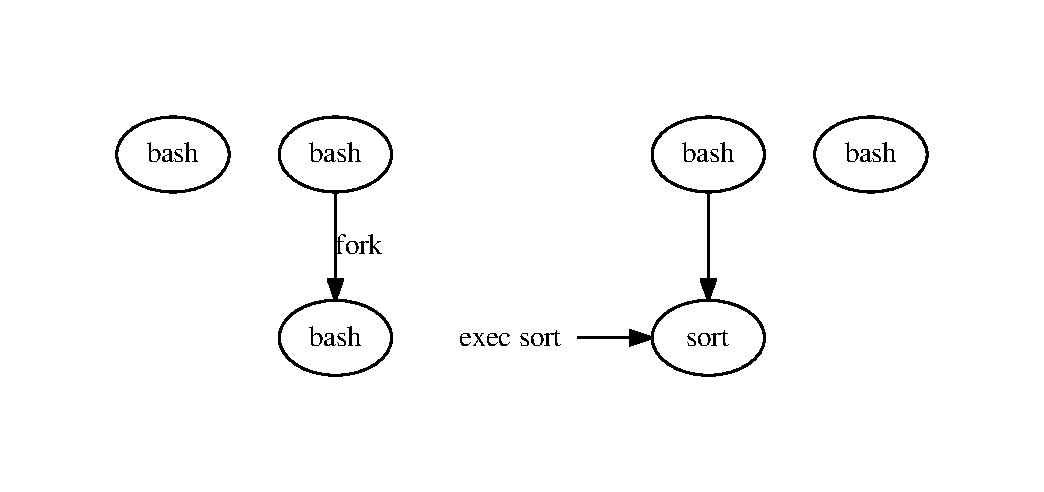
\includegraphics[width=.9\linewidth]{img/fork-exec.pdf}
\end{itemize} % ends low level
\end{frame}
\begin{frame}
\frametitle{shell脚本的执行过程}
\label{sec-1-3-2}
\begin{itemize}

\item 当前shell创建一个子shell并让子shell依次执行shell脚本中的命令,子shell执行完脚本中所有命令后结束,父shell结束等待状态,开始重新执行。\\
\label{sec-1-3-2-1}%
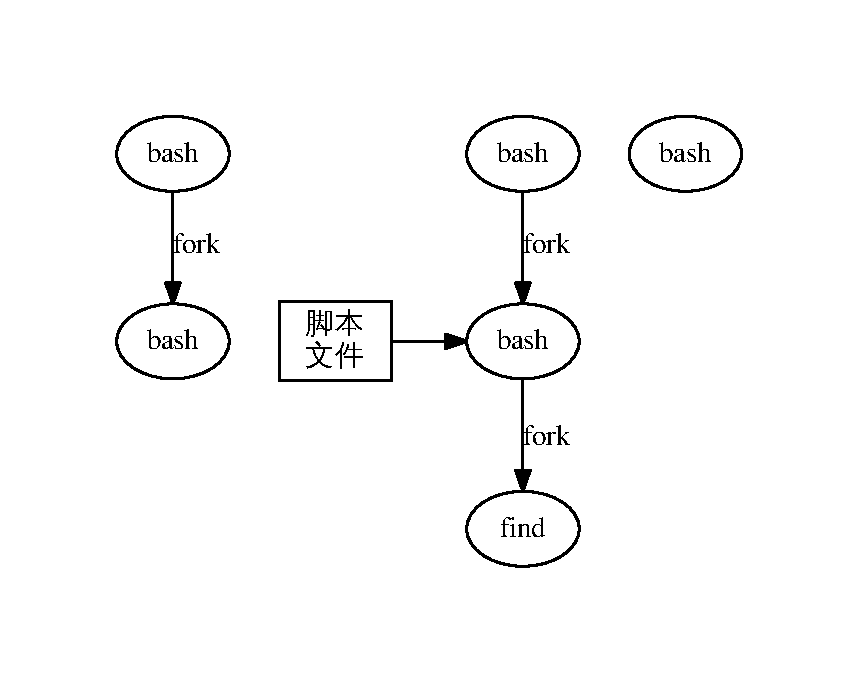
\includegraphics[width=.9\linewidth]{img/exec-shell.pdf}
\end{itemize} % ends low level
\end{frame}
\begin{frame}[fragile]
\frametitle{exec命令(1)}
\label{sec-1-3-3}
\begin{itemize}

\item 功能1:执行新进程并用新进程取代当前进程
\label{sec-1-3-3-1}%
\end{itemize} % ends low level
\begin{exampleblock}{示例}
\label{sec-1-3-3-2}


\begin{minted}[]{bash}
cat excmd
uname -a
exec date
echo “This line is never displayed”

exec_excmd #由于exec不返回到调用位置,因此其后的命令将无法执行。
\end{minted}
\end{exampleblock}
\end{frame}
\begin{frame}[fragile]
\frametitle{exec命令(2)}
\label{sec-1-3-4}
\begin{exampleblock}{功能2:打开和关闭文件描述符}
\label{sec-1-3-4-1}


\begin{minted}[]{bash}
#bash最多允许同时使用10个文件描述符(n=0~9)
exec [n=0]<file  #为标准输入重定向打开file
exec [n=1]>file  #为标准输出重定向(覆盖)打开file
exec [n=1]>>file #为标准输出重定向(追加)打开file
exec n<>file     #为标准输入输出重定向打开file
cmd <&n          #输入重定向到文件描述符n
cmd >&n          #输出重定向(覆盖)到文件描述符n
cmd >>&n         #输出重定向(追加)到文件表述符n
exec n>&m        #把m复制到n,将输出同时重定向到m和n
exec <&-         #关闭标准输入
exec >&-         #关闭标准输出
exec n<&-        #关闭重定向为标准输入的文件描述符n
exec n>&-        #关闭重定向为标准输出的文件描述符n
\end{minted}
\end{exampleblock}
\end{frame}
\begin{frame}[fragile]
\frametitle{exec命令(3)}
\label{sec-1-3-5}
\begin{exampleblock}{diff2:比较两个文本文件是否内容相同}
\label{sec-1-3-5-1}


\begin{minted}[]{bash}
#!/bin/bash
if [ "$#" -ne 2 ]; then
  echo "usage: `basename $0` file1 file2" 1>&2; exit 1
elif [ ! -f "$1" ]; then
  echo "$1 is not a regular file" 1>&2; exit 2
elif [ ! -f "$2" ]; then
  echo "$2 is not a regular file" 1>&2; exit 3
fi
\end{minted}
\end{exampleblock}
\end{frame}
\begin{frame}[fragile]
\frametitle{exec命令(4)}
\label{sec-1-3-6}
\begin{exampleblock}{diff2:(续1)}
\label{sec-1-3-6-1}


\begin{minted}[]{bash}
file1="$1"; file2="$2"; i=1
exec 3<"$file1"; exec 4<"$file2"
while read line1 0<&3; do
  if read line2 0<&4; then
    if [ "$line1" != "$line2" ]; then
      echo "different at line $i" 1>&2; exit 1
    fi
  else
    echo "$file1 is longer than $file2" 1>&2; exit 2
  fi
  ((i++))
done
\end{minted}
\end{exampleblock}
\end{frame}
\begin{frame}[fragile]
\frametitle{exec命令(5)}
\label{sec-1-3-7}
\begin{exampleblock}{diff2:(续2)}
\label{sec-1-3-7-1}


\begin{minted}[]{bash}
if read line2 0<&4; then
  echo "$file1 is shorter than $file2" 1>&2; exit 3
else
  echo "$file1 and $file2 are the same"; exit 0
fi
exec 3<&-; exec 4<&-

diff2 file1 file2
\end{minted}
\end{exampleblock}
\end{frame}
\begin{frame}[fragile]
\frametitle{trap命令(1)}
\label{sec-1-3-8}
\begin{itemize}

\item trap用于捕捉信号并指定收到信号时所执行的操作。
\label{sec-1-3-8-1}%
\end{itemize} % ends low level
\begin{exampleblock}{示例}
\label{sec-1-3-8-2}


\begin{minted}[]{bash}
trap -l #查看信号列表,同kill -l
trap 'echo "Ctrl-C disabled."' 2 #捕获信号2并执行指定命令
trap -p #查看当前信号捕获情况
trap    #同上
trap '' TERM INT #捕获并忽略信号2和15
trap - 1 2 15    #恢复信号1,2,15的系统默认处理
trap 1 2 15      #同上
\end{minted}
\end{exampleblock}
\begin{block}{注意}
\label{sec-1-3-8-3}


\begin{verbatim}
1. 比较重要的、能够捕捉的常用信号:0,1,2,3,15,20
2. 不能捕捉2个信号:9,19
3. 不应捕捉4个信号:10,12,17,30
\end{verbatim}
\end{block}
\end{frame}
\begin{frame}[fragile]
\frametitle{trap命令(2)}
\label{sec-1-3-9}
\begin{exampleblock}{leave:短暂离开时锁住终端}
\label{sec-1-3-9-1}


\begin{minted}[]{bash}
#!/bin/bash
#锁屏
trap '' 1 2 3 15 20  #忽略信号
clear
stty -echo           #关闭回显
echo -e "Enter your password: \c"
read pass1
echo -e "\nEnter your password again: \c"
read pass2
if [ "$pass1" != "$pass2" ]; then
  echo "Passwords do not match." 1>&2
  stty echo          #恢复回显
  exit 1
fi
\end{minted}
\end{exampleblock}
\end{frame}
\begin{frame}[fragile]
\frametitle{trap命令(3)}
\label{sec-1-3-10}
\begin{exampleblock}{leave:(续)}
\label{sec-1-3-10-1}


\begin{minted}[]{bash}
#解锁
until [ "$code" = "$pass1" ]; do
  clear
  echo -n "Enter the password: "
  read code
done
clear
echo 'Welcome back!'
stty echo            #恢复回显
exit 0
\end{minted}
\end{exampleblock}
\end{frame}
\begin{frame}[fragile]
\frametitle{eval命令(1)}
\label{sec-1-3-11}
\begin{itemize}

\item eval args\ldots{}\\
\label{sec-1-3-11-1}%
eval将所有参数合成一个字符串,并将得到的字符串作为命令执行。
\end{itemize} % ends low level
\begin{exampleblock}{示例1}
\label{sec-1-3-11-2}


\begin{minted}[]{bash}
x=100; y=x
echo $y
echo '$'$y
eval echo '$'$y #等价于echo $x,同echo ${!y}
eval $y=200     #等价于x=200
echo $x
\end{minted}
\end{exampleblock}
\begin{block}{lastarg:打印传递给脚本的最后一个参数}
\label{sec-1-3-11-3}


\begin{minted}[]{bash}
#!/bin/bash
eval echo '$'$#
\end{minted}
\end{block}
\end{frame}
\begin{frame}[fragile]
\frametitle{echo高级输出(1)}
\label{sec-1-3-12}
\begin{exampleblock}{输出彩色字符和彩色背景}
\label{sec-1-3-12-1}


\begin{minted}[]{bash}
echo -e "\033[31;46mhello world\033[0m"
#\033代表ESC,而“ESC[参数m”可用来设置显示属性
#31-前景色为红色,46-背景色为青色
#0-恢复默认设置

#\033也可写成\e
echo -e "\e[33;44mhello world\e[0m"
#33-前景色为棕色,44-背景色为蓝色
\end{minted}
\end{exampleblock}
\end{frame}
\begin{frame}[fragile]
\frametitle{echo高级输出(2)}
\label{sec-1-3-13}
\begin{exampleblock}{常用显示属性值}
\label{sec-1-3-13-1}


\begin{minted}[]{bash}
0 恢复默认值
1 加粗
4 下划线
7 反白显示
30 黑色(前景)        40 黑色(背景)
31 红色(前景)        41 红色(背景)
32 绿色(前景)        42 绿色(背景)
33 棕色(前景)        43 棕色(背景)
34 蓝色(前景)        44 蓝色(背景)
35 品红(前景)        45 品红(背景)
36 青色(前景)        46 青色(背景)
37 白色(前景)        47 白色(背景)
man console_codes  #查看更多属性
\end{minted}
\end{exampleblock}
\end{frame}
\begin{frame}[fragile]
\frametitle{tput命令(1)}
\label{sec-1-3-14}
\begin{exampleblock}{tput命令可以通过terminfo数据库调用终端功能}
\label{sec-1-3-14-1}


\begin{minted}[]{bash}
bel     #响铃
cols    #打印屏幕列数
clear   #清屏
smso    #开始突出显示模式
rmso    #结束突出显示模式
smul    #开始下划线模式
rmul    #结束下划线模式
rev     #反白显示
ed      #从光标位置到屏幕底部清屏
el      #从光标位置到行尾清除字符
sgr0    #关闭所有属性
bold    #粗体显示
cup r c #把光标移到r行c列
\end{minted}
\end{exampleblock}
\end{frame}
\begin{frame}[fragile]
\frametitle{tput命令(2)}
\label{sec-1-3-15}
\begin{exampleblock}{示例}
\label{sec-1-3-15-1}


\begin{minted}[]{bash}
tput clear; tput cup 10 20; echo "hello"
bell=`tput bel`; echo $bell
line=`tput smul`; offline=`tput rmul`
tput clear
tput cup 10 20; echo "${line}hello${offline}"

ls
tput cup 5 0; tput ed

tput -S <<!
clear
cup 10 10
!
\end{minted}
\end{exampleblock}
\end{frame}
\begin{frame}[fragile]
\frametitle{选项与参数处理(1)}
\label{sec-1-3-16}
\begin{itemize}

\item getopts命令:解析命令行选项,检查选项合法性。
\label{sec-1-3-16-1}%
\end{itemize} % ends low level
\begin{exampleblock}{示例:handleopts}
\label{sec-1-3-16-2}


\begin{minted}[]{bash}
cat handleopts
#!/bin/bash
while getopts o:r:nt opt; do
  case "$opt" in
    o) output_file="$OPTARG";;
    r) report_file="$OPTARG";;
    n) number_option="yes";;
    t) title="no";;
    *) exit 1;
  esac
done
\end{minted}
\end{exampleblock}
\end{frame}
\begin{frame}[fragile]
\frametitle{选项与参数处理(2)}
\label{sec-1-3-17}
\begin{exampleblock}{示例:handleopts(续)}
\label{sec-1-3-17-1}


\begin{minted}[]{bash}
echo "Output_file = $output_file"
echo "Report_file = $report_file"
echo "Number_option = ${number_option:-no}"
echo "Title = ${title:-yes}"
echo "Arguments before shift: $*"
shift `expr $OPTIND - 1`
echo "Arguments after shift: $*"
exit 0
\end{minted}
\end{exampleblock}
\end{frame}
\begin{frame}
\frametitle{选项与参数选项(3)}
\label{sec-1-3-18}
\begin{exampleblock}{说明}
\label{sec-1-3-18-1}

\begin{enumerate}
\item while循环通过调用getopts每次获取一个选项并存入字符串变量opt中,直至读取不到新的选项或读取到--选项。
\item o:r:nt  表示接受4个选项,其中o和r带选项参数
\item \$OPTARG 表示当前选项的参数
\item \$OPTIND 指向第一个非选项参数的位置参数,即第一个命令参数。如果位置参数的值为--,则忽略之。
\end{enumerate}
\end{exampleblock}
\end{frame}
\begin{frame}[fragile]
\frametitle{选项与参数处理(4)}
\label{sec-1-3-19}
\begin{exampleblock}{测试:handleopts}
\label{sec-1-3-19-1}


\begin{minted}[]{bash}
handleopts -tn -o file.out -r file.rep unit.txt
handleopts -tn *
handleopts unit.txt
handleopts -tn -o file.out -r
\end{minted}
\end{exampleblock}
\end{frame}
\begin{frame}[fragile]
\frametitle{给awk传递参数(1)}
\label{sec-1-3-20}
\begin{exampleblock}{field n:打印输入的第n个字段}
\label{sec-1-3-20-1}


\begin{minted}[]{bash}
cat field1
#!/bin/bash
awk "{ print \$ $1 }"  #必须用双引号(两个$本应紧挨着)

cat field2
#!/bin/bash
awk '{ print $'$1' }'

who | field1 1
who | field2 2
\end{minted}
\end{exampleblock}
\end{frame}
\begin{frame}[fragile]
\frametitle{给awk传递参数(2)}
\label{sec-1-3-21}
\begin{block}{addup n:将输入的第n列求和}
\label{sec-1-3-21-1}


\begin{minted}[]{bash}
cat addup n
#!/bin/bash
awk '{ s+=$'$1' }
  END{ print s }'

cat score.list | addup 2
\end{minted}
\end{block}
\end{frame}
\begin{frame}[fragile]
\frametitle{给awk传递参数(3)}
\label{sec-1-3-22}
\begin{exampleblock}{sumup m n:将输入的第m至n列分别求和,并累加这些和}
\label{sec-1-3-22-1}


\begin{minted}[]{bash}
cat sumup
#!/bin/bash
awk '
BEGIN { m='$1'; n='$2' }
      { for (i=m; i<=n; i++) sum[i]+=$i }
  END { for (i=m; i<=n; i++) {
          printf("sum[%d] = %d\n", i, sum[i])
          total += sum[i]
          }
        printf("total = %d\n", total)
      }'

sumup 2 5 <score.list
\end{minted}
\end{exampleblock}
\end{frame}
\begin{frame}[fragile]
\frametitle{命令组}
\label{sec-1-3-23}
\begin{exampleblock}{( cmd1;cmd2;\ldots{} ) 在子shell中执行}
\label{sec-1-3-23-1}


\begin{minted}[]{bash}
x=3
(y=5; let x+=y; echo $x)
echo $x
\end{minted}
\end{exampleblock}
\begin{block}{\{ cmd1;cmd2;\ldots{}; \} 在当前shell中执行}
\label{sec-1-3-23-2}


\begin{minted}[]{bash}
x=3
{ y=5; let x+=y; echo $x; } #注意空格与分号
echo $x
\end{minted}
\end{block}
\end{frame}
\begin{frame}[fragile]
\frametitle{脚本调试(1)}
\label{sec-1-3-24}
\begin{exampleblock}{shell的-v和-x选项}
\label{sec-1-3-24-1}


\begin{verbatim}
-v选项: shell将显示每条原始命令及其执行结果。
-x选项: shell将显示每条扩展后的命令行及其执行结果。
\end{verbatim}
\end{exampleblock}
\begin{block}{示例}
\label{sec-1-3-24-2}


\begin{minted}[]{bash}
cat hour
#!/bin/bash
h=`date +%H`
echo $h

sh -v hour
sh -x hour
\end{minted}
\end{block}
\end{frame}
\begin{frame}[fragile]
\frametitle{脚本调试(2)}
\label{sec-1-3-25}
\begin{exampleblock}{在脚本内部开启和关闭调试}
\label{sec-1-3-25-1}


\begin{verbatim}
set -v/x: 开启调试
set +v/x: 关闭调试
\end{verbatim}
\end{exampleblock}
\begin{block}{示例}
\label{sec-1-3-25-2}


\begin{minted}[]{bash}
cat hour2
#!/bin/bash
set -v   #开启调试
h=`date +%H`
set +v   #关闭调试
echo $h
\end{minted}
\end{block}
\end{frame}
\begin{frame}
\frametitle{脚本调试(3)}
\label{sec-1-3-26}
\begin{itemize}

\item 利用trap命令进行调试(1)
\label{sec-1-3-26-1}%
\begin{itemize}

\item 伪信号:由shell产生的信号,信号则是由操作系统产生的
\label{sec-1-3-26-1-1}%
\end{itemize} % ends low level

\item 伪信号列表\\
\label{sec-1-3-26-2}%
\begin{center}
\begin{tabular}{ll}
 伪信号   &  产生时机                             \\
\hline
 EXIT(0)  &  从函数或脚本中退出                   \\
 RETURN   &  调用函数后或用.命令执行其他脚本之后  \\
 ERR      &  某条命令返回非0状态(不成功)时        \\
 DEBUG    &  脚本中每条命令执行之前               \\
\end{tabular}
\end{center}


\end{itemize} % ends low level
\end{frame}
\begin{frame}[fragile]
\frametitle{脚本调试(4)}
\label{sec-1-3-27}
\begin{itemize}

\item 利用trap命令进行调试(2)
\label{sec-1-3-27-1}%
\end{itemize} % ends low level
\begin{exampleblock}{示例1:trap-debug1}
\label{sec-1-3-27-2}


\begin{minted}[]{bash}
#!/bin/bash
trap 'echo "EXIT: min=$min max=$max"' EXIT
min=$1
max=$2
if [ $min -gt $max ]; then
  exit 1
fi

trap-debug1 6 8
\end{minted}
\end{exampleblock}
\end{frame}
\begin{frame}[fragile]
\frametitle{脚本调试(5)}
\label{sec-1-3-28}
\begin{itemize}

\item 利用trap命令进行调试(3)
\label{sec-1-3-28-1}%
\end{itemize} % ends low level
\begin{exampleblock}{示例2:trap-debug2}
\label{sec-1-3-28-2}


\begin{minted}[]{bash}
#!/bin/bash
trap 'echo "ERR($LINENO): name=$name"' ERR
name=`grep william /etc/passwd`
exit 0

trap-debug2
\end{minted}
\end{exampleblock}
\end{frame}
\begin{frame}[fragile]
\frametitle{脚本调试(6)}
\label{sec-1-3-29}
\begin{itemize}

\item 利用trap命令进行调试(4)
\label{sec-1-3-29-1}%
\end{itemize} % ends low level
\begin{exampleblock}{示例3:trap-debug3}
\label{sec-1-3-29-2}


\begin{minted}[]{bash}
#!/bin/bash
trap 'echo "DEBUG($LINENO): var=$var"' DEBUG
var=29
let var=var*2
exit 0

trap-debug3
\end{minted}
\end{exampleblock}
\end{frame}
\begin{frame}[fragile]
\frametitle{脚本调试(7)}
\label{sec-1-3-30}
\begin{itemize}

\item 可以结合调试变量和echo语句进行调试
\label{sec-1-3-30-1}%
\end{itemize} % ends low level
\begin{exampleblock}{示例}
\label{sec-1-3-30-2}


\begin{minted}[]{bash}
cat sum2n
#!/bin/bash
n=${1:-100}
for i in $(seq $n); do
  let sum+=i
  [ "$debug" = "on" ] && echo "DEBUG: i=$i sum=$sum"
done
echo "1+...+$n=$sum"

sum2n 10             #正常运行
debug=on sum2n 10    #调试运行
\end{minted}
\end{exampleblock}
\end{frame}
\begin{frame}[fragile]
\frametitle{综合实例}
\label{sec-1-3-31}
\begin{itemize}

\item 个人书籍管理系统
\label{sec-1-3-31-1}%
\end{itemize} % ends low level
\begin{exampleblock}{书籍信息字段}
\label{sec-1-3-31-2}


\begin{verbatim}
ID        #编号 (5位数字,如00023)
Title     #书名
Author    #作者
Class     #类别 (os-operating system
                se-software engineering
                pl-programming language
                cn-computer networks
                db-database
                ob-other books)
state     #状态 (in-未借出,out-已借出)
bname     #借阅人
btime     #借出时间
\end{verbatim}
\end{exampleblock}
\end{frame}
\begin{frame}
\frametitle{shell编程实践}
\label{sec-1-3-32}
\begin{block}{试一试}
\label{sec-1-3-32-1}

\begin{enumerate}
\item 请试一试完善和改进现有个人书籍管理系统
\item 请试一试用shell开发一个其他信息管理系统
\end{enumerate}
\end{block}
\end{frame}

\end{document}
